% Options for packages loaded elsewhere
\PassOptionsToPackage{unicode}{hyperref}
\PassOptionsToPackage{hyphens}{url}
\documentclass[
  11pt,
  fontset=fandol]{ctexart}
\usepackage{xcolor}
\usepackage[margin=2cm]{geometry}
\usepackage{amsmath,amssymb}
\setcounter{secnumdepth}{-\maxdimen} % remove section numbering
\usepackage{iftex}
\ifPDFTeX
  \usepackage[T1]{fontenc}
  \usepackage[utf8]{inputenc}
  \usepackage{textcomp} % provide euro and other symbols
\else % if luatex or xetex
  \usepackage{unicode-math} % this also loads fontspec
  \defaultfontfeatures{Scale=MatchLowercase}
  \defaultfontfeatures[\rmfamily]{Ligatures=TeX,Scale=1}
\fi
\usepackage{lmodern}
\ifPDFTeX\else
  % xetex/luatex font selection
\fi
% Use upquote if available, for straight quotes in verbatim environments
\IfFileExists{upquote.sty}{\usepackage{upquote}}{}
\IfFileExists{microtype.sty}{% use microtype if available
  \usepackage[]{microtype}
  \UseMicrotypeSet[protrusion]{basicmath} % disable protrusion for tt fonts
}{}
\makeatletter
\@ifundefined{KOMAClassName}{% if non-KOMA class
  \IfFileExists{parskip.sty}{%
    \usepackage{parskip}
  }{% else
    \setlength{\parindent}{0pt}
    \setlength{\parskip}{6pt plus 2pt minus 1pt}}
}{% if KOMA class
  \KOMAoptions{parskip=half}}
\makeatother
\setlength{\emergencystretch}{3em} % prevent overfull lines
\providecommand{\tightlist}{%
  \setlength{\itemsep}{0pt}\setlength{\parskip}{0pt}}
\usepackage{float}
\usepackage{caption}
\usepackage{tikz,pgfplots}
\usepackage{hyperref}
\pgfplotsset{compat=1.18}
\usepgfplotslibrary{groupplots}
\hypersetup{colorlinks=true,linkcolor=blue!50!black,urlcolor=blue!50!black}
\setlength{\emergencystretch}{3em}
\setlength{\parskip}{0.4em}
\pagestyle{plain}
\usepackage{bookmark}
\IfFileExists{xurl.sty}{\usepackage{xurl}}{} % add URL line breaks if available
\urlstyle{same}
\hypersetup{
  pdftitle={中文导读：更新哪些层，模型能多找到哪些核？},
  hidelinks,
  pdfcreator={LaTeX via pandoc}}

\title{中文导读：更新哪些层，模型能多找到哪些核？}
\author{}
\date{2026-11-15}

\begin{document}
\maketitle

{
\setcounter{tocdepth}{2}
\tableofcontents
}
本阶段把模型的训练改变拆成多个固定对照：扩大输入、额外类别监督、平均参数、限制参数移动，以及更新编码器不同位置的层。每项都重新训练同轮对照，再统计预测中心与标注核的一对一匹配。详细数据和协议见
\href{../RESULTS_ZH.md}{中文分析}。

最值得关注的是三条证据。更新全部 24 层时，两个种子都多找到了较多 Dead
核；只更新前十二层时，模型减少了许多额外预测；把十二层交错分布到整个编码器，虽然提高了总体匹配，Dead
改善却很小。这说明``多训练一些参数''与``在哪些位置更新''需要分别比较，训练集上找到更多核也不能单独预测开发集的改善。

\begin{figure}[H]\centering
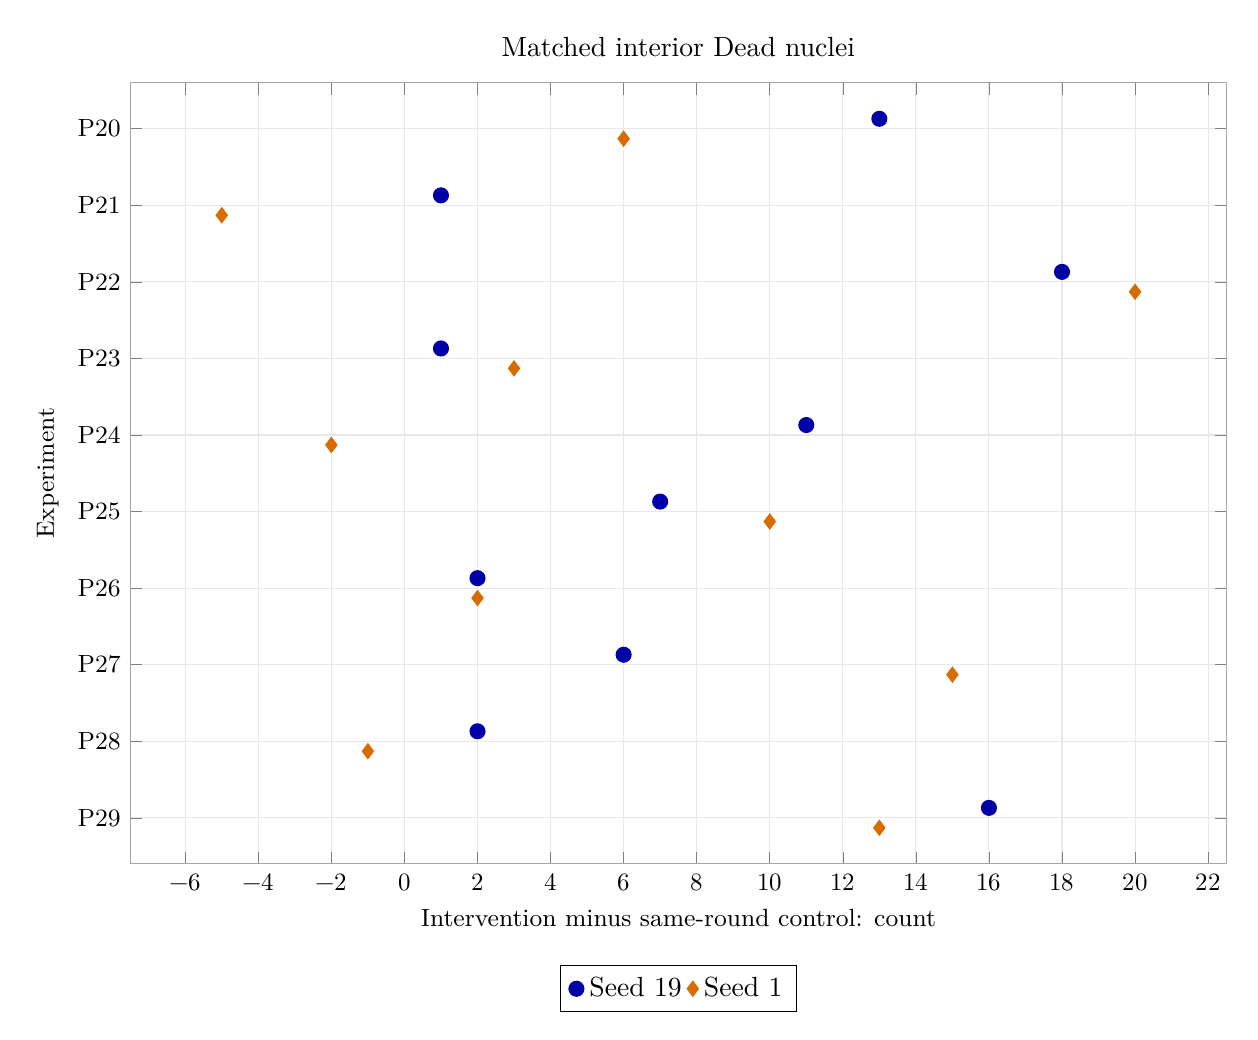
\begin{tikzpicture}
\begin{axis}[width=15.5cm,height=11.5cm,xlabel={Intervention minus same-round control: count},ylabel={Experiment},title={Matched interior Dead nuclei},ytick={0,1,2,3,4,5,6,7,8,9},yticklabels={P20,P21,P22,P23,P24,P25,P26,P27,P28,P29},ymin=-.6,ymax=9.6,y dir=reverse,grid=major,grid style={gray!18},legend style={at={(.5,-.13)},anchor=north,legend columns=2},axis line style={gray!70},tick label style={font=\small},label style={font=\small},title style={font=\normalsize}]
\addplot[only marks,mark=*,mark size=2.7pt,color=blue!65!black] coordinates {(13,-0.13) (1,0.87) (18,1.87) (1,2.87) (11,3.87) (7,4.87) (2,5.87) (6,6.87) (2,7.87) (16,8.87)};
\addlegendentry{Seed 19}
\addplot[only marks,mark=diamond*,mark size=2.7pt,color=orange!85!black] coordinates {(6,0.13) (-5,1.13) (20,2.13) (3,3.13) (-2,4.13) (10,5.13) (2,6.13) (15,7.13) (-1,8.13) (13,9.13)};
\addlegendentry{Seed 1}
\end{axis}
\end{tikzpicture}

\caption{阶段内部 Dead 匹配变化}
\end{figure}

最新 P29 更新前六层和后六层。种子 19/1 分别多找到 16/13 个内部 Dead
核，召回从 44.83\%/46.21\% 提高到 55.86\%/55.17\%；总匹配增加
283/165，额外点减少 65/64。两个种子的配对区间均为正，最终 Dead
召回和精度仍低于原定要求，原双种子完整条件未通过。下一轮固定比较中间十二层与最后十二层，补上连续层位置的对照。

\noindent

\begin{minipage}{\linewidth}\centering
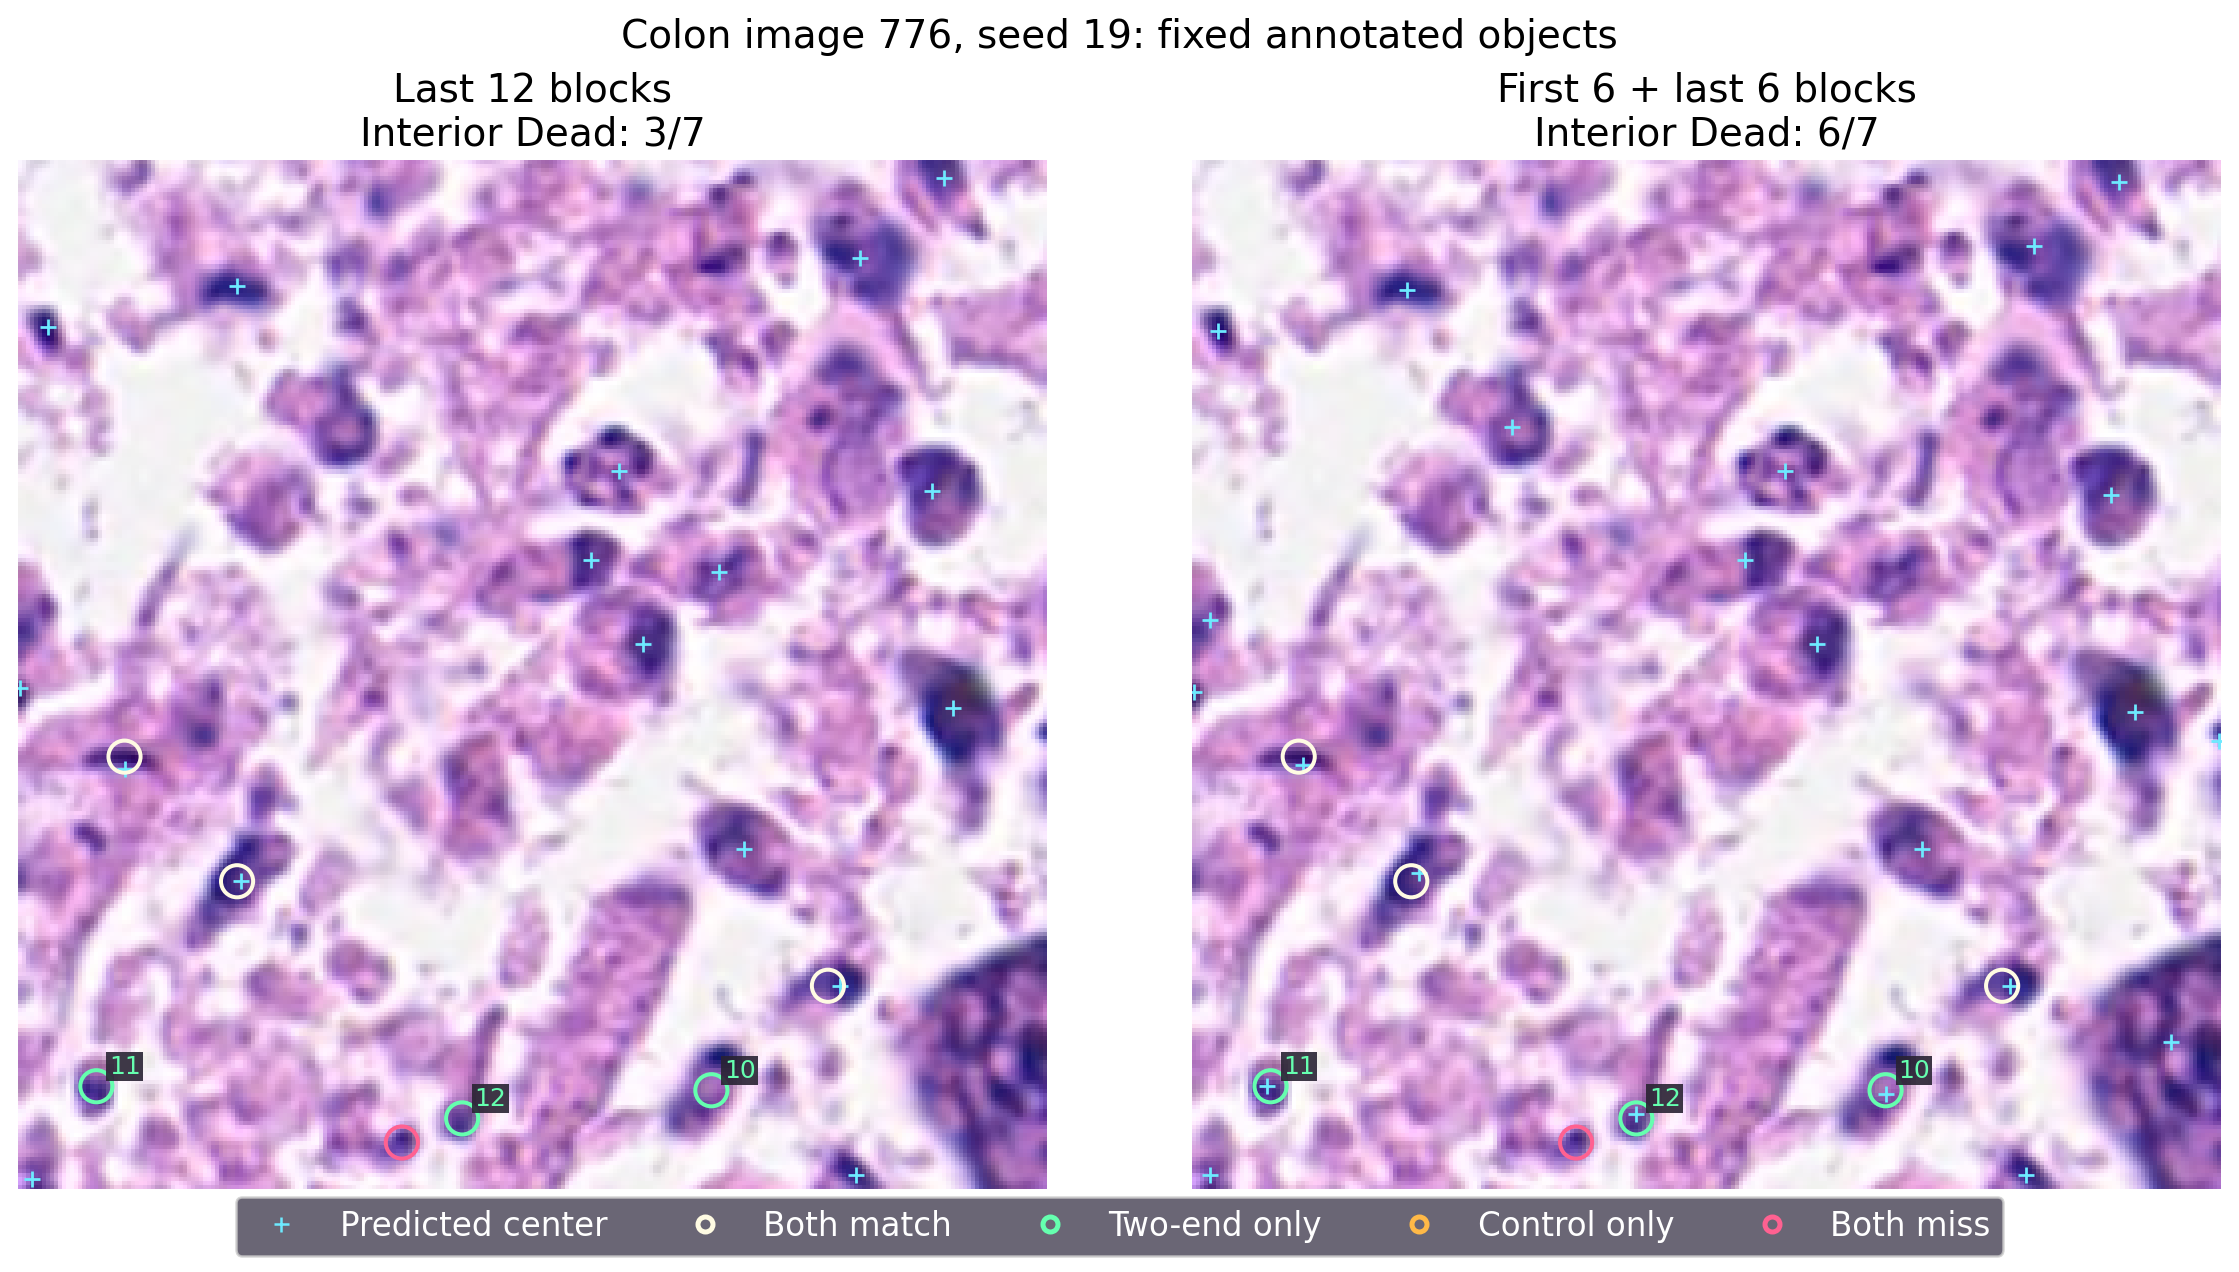
\includegraphics[width=\linewidth,height=0.40\textheight,keepaspectratio]{../figures/p29_image_776_seed_19.png}
\captionof{figure}{结肠固定样例}
\raggedright

先看结肠图像下方编号 10、11、12 的绿色圆圈。右图三个标注附近都有青色预测十字，左图附近没有预测。三个最近点距离从约 41、28、81 像素降至 1 像素，目标匹配从 3 个增加到 6 个。这是具体核被找回的可核查例子。

\end{minipage}

\noindent

\begin{minipage}{\linewidth}\centering
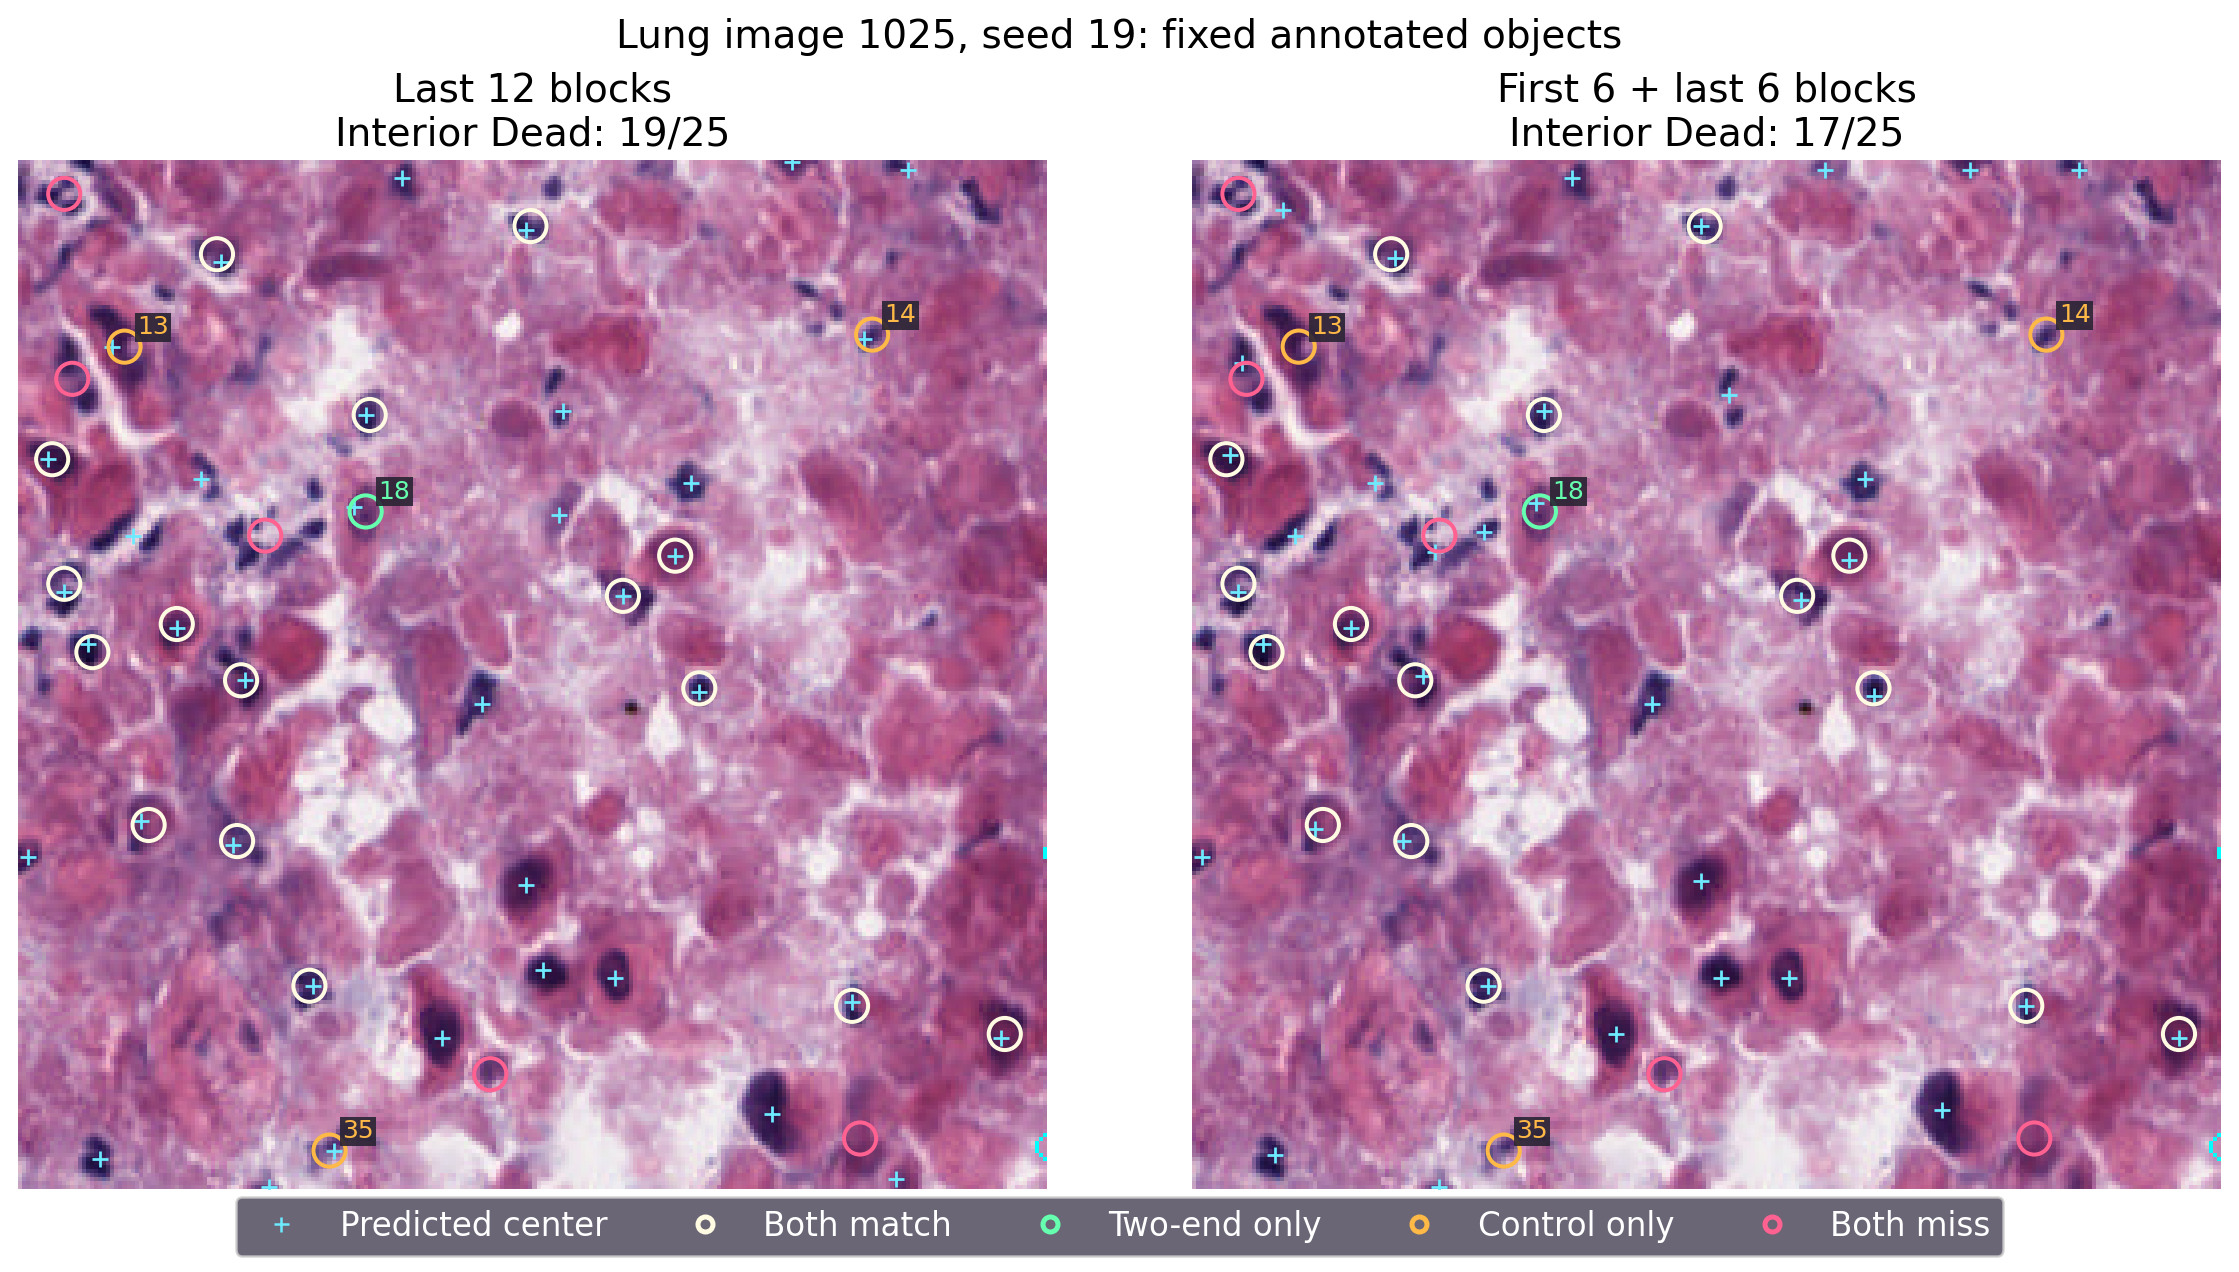
\includegraphics[width=\linewidth,height=0.40\textheight,keepaspectratio]{../figures/p29_image_1025_seed_19.png}
\captionof{figure}{肺组织固定样例}
\raggedright

再看肺组织图像 1025：它整体少找到两个 Dead 核。新增一个匹配的同时，三个原来有匹配的核失去了附近预测，其中一个面积只有 31 像素。改善不是每张组织图都同方向。详细报告逐一给出这些核的坐标和距离，并讨论“附近新增输出”和“点移动跨越三像素匹配半径”两种可观察事件。

\end{minipage}

固定八张样例中的 Dead 核净增加两个，完整 522 张开发评估图像净增加 16
个。样例用于解释具体发生了什么，完整数据用于确定改善幅度。肺组织图像
1038 和食管图像 2076 贡献了 10
个净增加量；逐一去掉一张阳性图像的敏感性分析仍保持正方向。结果图、原始坐标和数值表都已保存，可以复查图中的每个变化。

本阶段使用反复分析的第 1
折开发数据，采用最后检查点和固定中心匹配规则。后续机制分析还需要模型概率图或隐层测量，才能分清点的变化来自分数、峰值筛选还是表征改变。

\noindent

\begin{minipage}{\linewidth}\centering
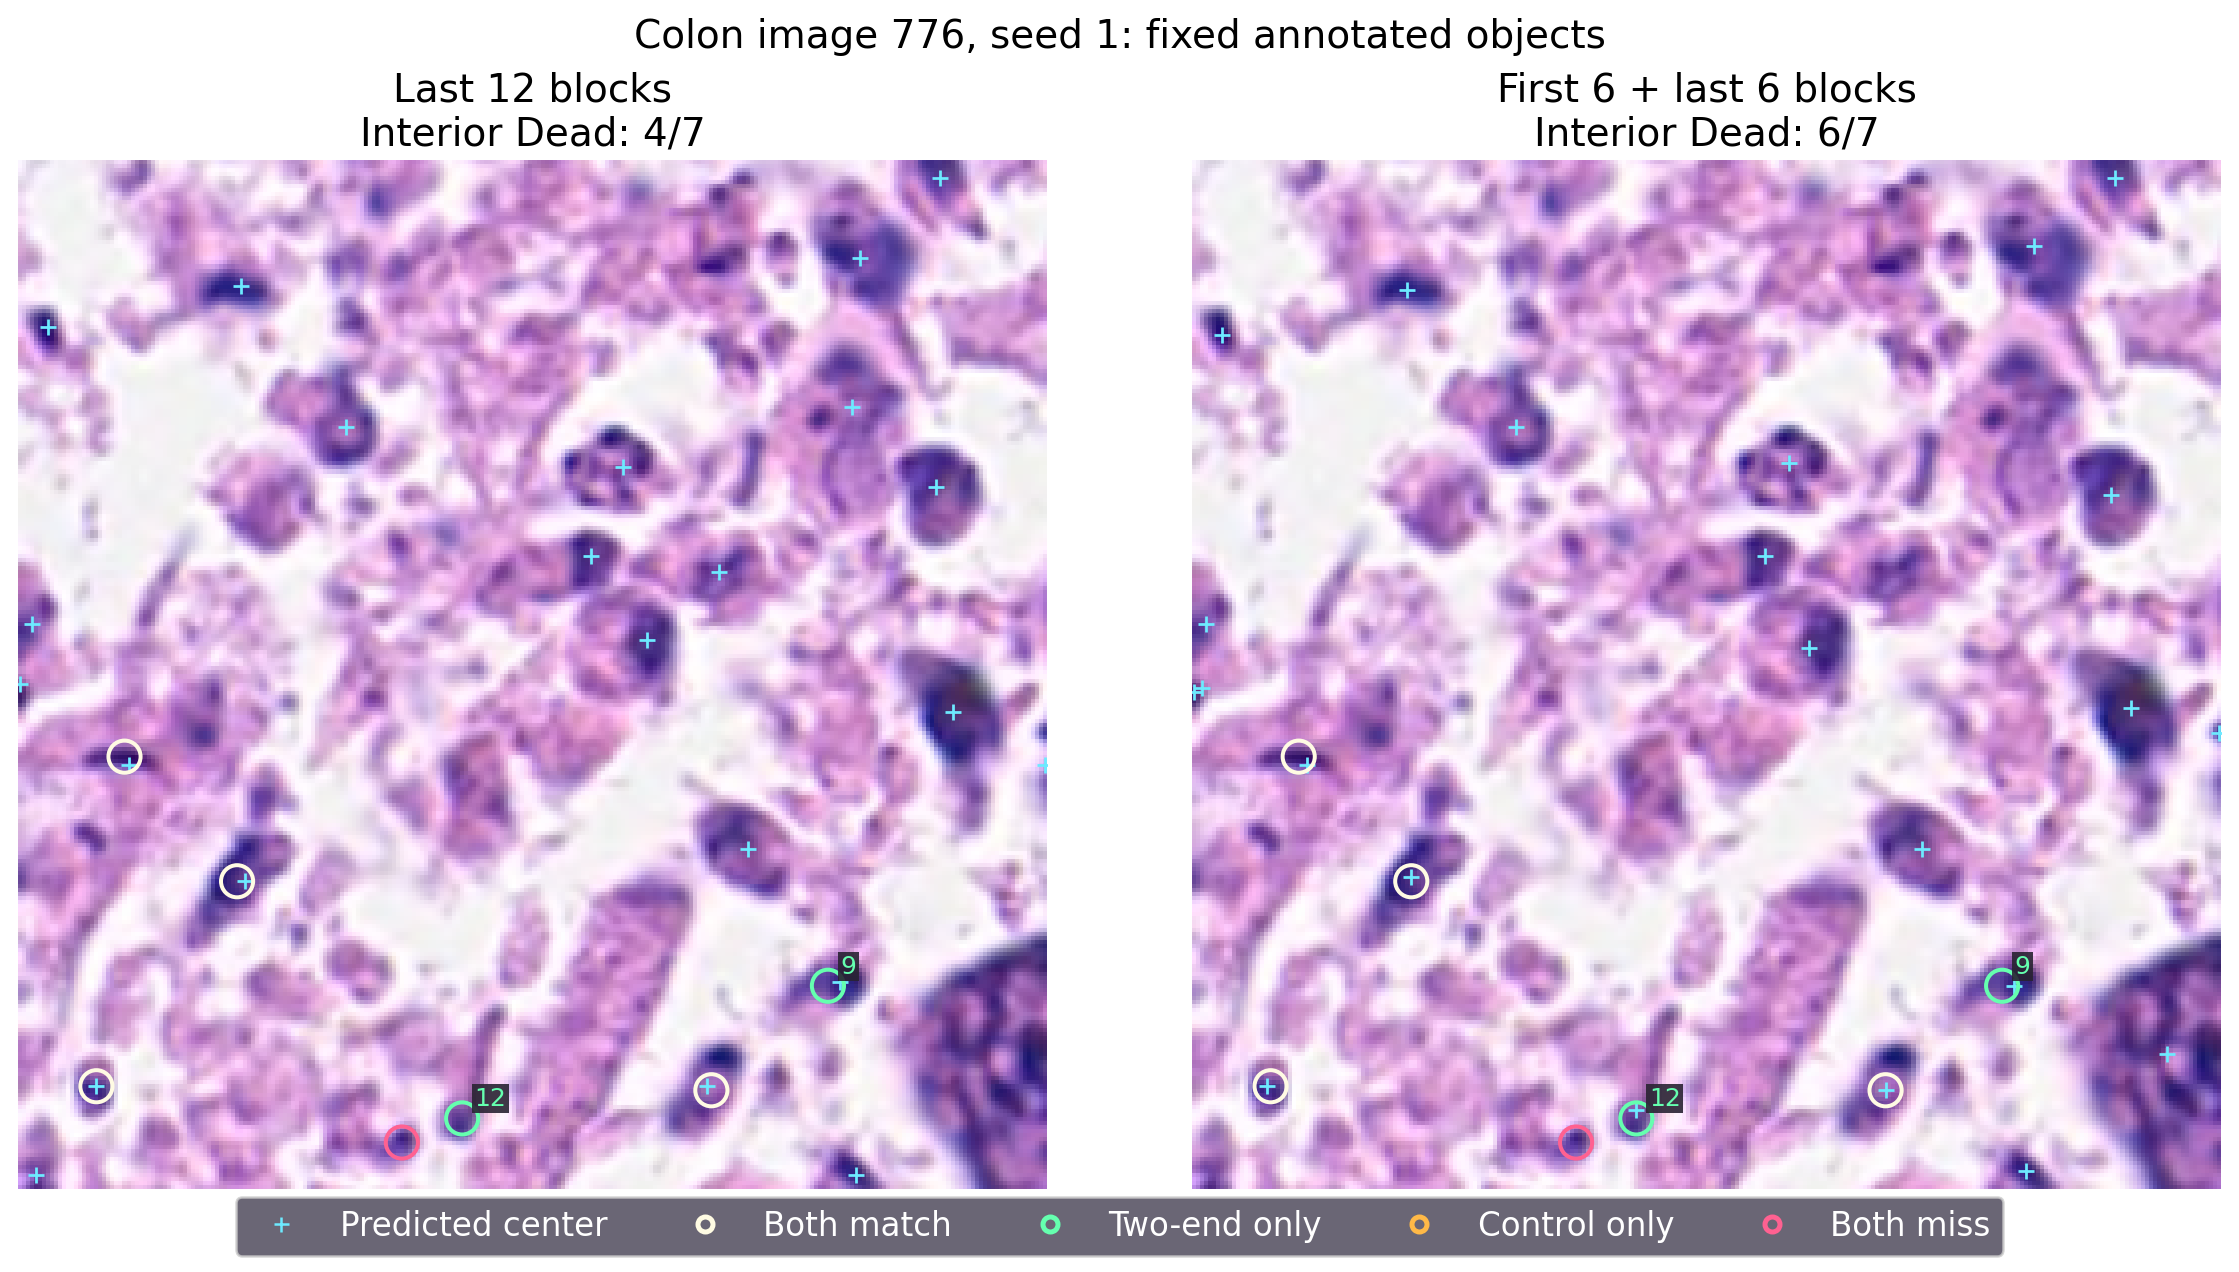
\includegraphics[width=\linewidth,height=0.40\textheight,keepaspectratio]{../figures/p29_image_776_seed_1.png}
\captionof{figure}{种子 1 的结肠图像}
\raggedright

两个种子是否找回了同一个核，也可以直接复查：结肠对象 12 位于（238，110），两个实验模型都在它附近新增有效预测。肺组织图像 1025 的对象 35 则在两个种子中都丢失了匹配。另一张肺组织图像 1037 在种子 1 的匹配总数不变，却交换了两个新增和两个丢失。详细报告把重复恢复、重复丢失和局部交换分开解释，而不只比较图像总数。

\end{minipage}

四个模型的训练与开发评估已完成。实验种子 1 的作业在保存阶段超时后，CPU
恢复作业完整保存了两个检查点和 12
张最终图片，并核验源文件与目标回读哈希；完整交付包含 48
张最终模型结果图和 13 张分析图。下一轮 P30 已冻结，正式提交的实际状态见
\href{../P30_SUBMISSION.md}{P30 记录}。

\end{document}
